\chapter{绪论}
\label{cha:intro}

\section{研究背景}%2
在软件开发过程中,代码错误的发现与修正贯穿始终。近年来大量错误检测工具(如静态分析工具、动态分析工具、代码验证工具、测试管理工具等%TODO:cite
)在工业界得到了较好的应用,这些工具大大提高了开发人员发现代码错误的效率,然而这些错误仍然需要人工分析和修复。研究表明,错误的定位与修复最高可占用软件开发过程中70\%的时间。%TODO:cite{!!!}。
如何在错误修复这一环节提供工具支持并提高效率已成为软件工程研究的重要内容。

基于“生成-检验”框架的错误自动修复技术是众多错误修复技术中的一个分支。该技术从程序源代码出发,以源码自带的测试集是否通过为判别程序正确与否的标准,试图生成针对源码的修改建议,使应用该建议修改后的程序能够通过测试集,从而达到修复错误的目的。
\begin{figure}[!h]
	\centering
	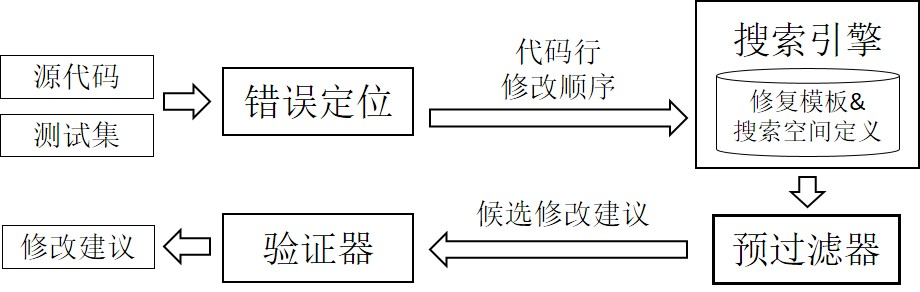
\includegraphics[width=0.7\linewidth]{chap01/general-structure}
	\caption{研究思路}
	\label{fig:general-structure}
\end{figure}

图\ref{fig:general-structure}展示了“生成-检验”框架的一般结构和工作流程。如图所示,“生成-检验”系统的输入包括程序源代码、测试代码和测试结果(如通过、不通过、错误路径等),内部共包含“错误定位器”,“搜索引擎”和“检验器”三个主要模块,分别对应“错误定位”、“变体生成”和“修复检验”三个主要工作步骤,最终系统输出一系列可能的修改建议,使得源代码经修改后可以通过测试代码中的测试。具体而言,首先,错误定位器将分析程序的运行轨迹,找出源代码中与测试错误相关的部分,称为“可修改位置”,并将各个位置按照出错的可能性由高到底排序,形成“可修改位置”列表。接着,搜索引擎按照这一列表由高到低的顺序针对各个位置生成可能的代码修改方案。最终,检验器将这些修改方案逐一应用到源代码中,重新编译并执行测试代码。当测试代码通过时,被检验的修改方案输出给开发人员,通过人工判断决定采用哪一种修改方案。

\begin{lstlisting}[caption=“生成-检验”框架应用示例,frame=single,language=Java,numbers=left,basicstyle=\ttfamily\footnotesize,label=code:example-src]
public class Calculator {
  public int add (int a, int b) {
    return a + b;
  }
  public int minus (int a, int b) {
    return a + b; // Error: should be (a - b)
  }
}
\end{lstlisting}

\begin{lstlisting}[caption=“生成-检验”框架应用示例,frame=single,language=Java,numbers=left,basicstyle=\ttfamily\footnotesize,label=code:example-test]
public class CalculatorTest {  
  @Test
  public void testAdd () {
    Calculator cal = new Calculator();
    int a = 1;
    int b = 2;
    Assert.assertEquals(3, cal.add(a, b));
  }  
  @Test
  public void testMinus (int a, int b) {
    Calculator cal = new Calculator();
    int a = 1;
    int b = 2;
    Assert.assertEquals(-1, cal.minus(a, b));
  }  
}
\end{lstlisting}

例如,代码\ref{code:example-src}与代码\ref{code:example-test}
展示了一个简单Java程序的源代码。主程序包含一个类Calculator,并提供两个公有方法add和minus,分别处理加、减两种操作。类Calculator对应的JUnit单元测试类CalculatorTest包含两个测试方法,分别测试加、减两种操作的正确性。读代码可知,代码\ref{cha:code:example-src}第6行中返回值表达式有一处错误:减法操作本应返回两个表达式相减,而实际返回了两个表达式相加。实际运行测试代码时也可看到,测试方法testMinus将在测试代码第16行触发AssertionFailureException,表示期望返回值(-1)与实际返回值(3)不符。

为修正这一错误,“生成-检验”系统将首先定位与异常发生相关的程序语句,此处即为主程序第6行。接着,系统将对第6行做合理的程序变换,例如将表达式 a + b 变为 a - b, a + 1, 1 + b, -a, -b...最后,系统将这些变换代回源代码,重新编译并执行测试,此时可发现若是用a - b或-a替换a + b,则两个测试用例均能够通过,因此两种修改方式均会提交给开发人员做人工判断。不难看出,将a + b替换为-a使测试集通过仅仅是巧合,正确的修改应当是替换为a - b。至此,程序错误被修复。


评价一个“生成-检验”系统的优劣应从两个维度出发。一是“正确率”,即在相同代码错误集合上能够成功修复的代码错误比例,二是“效率”,即修复同一代码错误所消耗的时间。从工作流程上看,如果不限时间,“生成-检验”系统的修复能力,即其所能够成功修复的错误范围完全由其搜索引擎中所包含的程序变体生成模板集合决定。模板集合越大,所能覆盖的程序错误范围越广,能够生成出正确修改方案的可能性就越高,系统正确率也越高。这使得“生成-检验”系统在理论上可以修正任何由测试集定义的代码错误而不局限于特定的错误类型。然而,由于程序变体数量巨大,实际的计算过程中难以穷尽,如何在保证一定的正确率前提下尽可能提高系统的效率成为了实际系统设计与实现中的重要问题,也是本文的中心内容。

错误定位算法、搜索引擎及检验器对系统效率具有如下影响:
\begin{enumerate}
	\item 错误定位的结果决定了源代码中发生错误的代码位置被搜索到的顺序,因此它也直接决定了系统将在生成一个正确的修改方案前所花费的时间。错误定位的结果越准确,耗费时间越少,效率越高。
	\item 搜索引擎中包含了一系列预定义的程序变体生成模板。对所有可能的代码修复位置,搜索引擎均会根据这些生成模板生成一系列的程序变体。由于所有修复方案均需要输入到检验器做测试,模板所覆盖的变体生成方案越多,检验过程消耗的时间也越长,效率也就随之降低。
	\item 在检验器检验一个备选修复方案是否能够使得源程序测试集通过时,源程序将被修改、重新编译并运行,这一过程将在编译、运行环节上耗费大量时间。因此检验器的设计和实现将直接影响系统的整体效率。
\end{enumerate}

基于以上分析,本文将从提高错误定位算法准确度、压缩搜索引擎的搜索空间、提高检验器检验修复方案等角度提高系统效率,优化系统设计,使“生成-检验”系统向实际应用更进一步。

\section{研究现状}%10

现有研究工作的研究内容可分为两大类。一是“生成-检验”框架中的某个具体工作步骤,即错误定位算法,修复建议生成算法及修复建议验证算法的研究。二是对“生成-检验”框架的整体改进。本节本文将对这几个方面的研究现状分别阐述。
\subsection{错误定位算法}
错误定位是“生成-检验”框架中的第一个计算步骤。事实上,错误定位算法成为一个独立的研究领域远早于“生成-检验”框架的提出。在本节我们将分为两个方面介绍错误定位算法的研究现状。

\textbf{算法设计:}错误定位算法的根本目的是根据程序的出错信息找到程序源代码中的错误位置,方便开发人员发现错误。根据算法的基本思想,现有的错误定位算法可以分为以下两大类。第一类是基于程序数据流、控制流分析的错误定位算法。这一类算法通常耗时较长,实现也稍显复杂,因此一般现有“生成-检验”系统常采用的是另一类算法,称作基于统计的错误定位算法(Spectrum-based Fault Localization,简称SFL算法)。

SFL算法根据程序测试集中测试用例的覆盖(Coverage)信息,依据“被越多的通过测试用例执行次数越多的语句越可能是正确的代码,被越多的不通过测试用例执行次数越多的语句越可能是错误的代码”这一经验规律,设计出一系列输入为执行次数,输出为程序语句错误的概率估计值的计算公式,最终根据该公式的计算结果按可疑值(Suspiciousness)由高到低排序,给出程序中最可能导致程序错误的语句列表。目前比较公认的计算公式是\cite{Abreu:2006:ESC:1193217.1194368},很多实验\cite{Yu:2008:ESE:1368088.1368116}\cite{Abreu20091780}都表明该公式给出的排序准确度能够稳定的超过其他公式。
SFL方法的优点是算法简单,速度快,并且由于很多语言已经提供了一定的插桩支持工具(如针对C语言的gcov,针对Java的JProfiler等)工程实现也比较容易。然而缺点也十分明显,由于经验公式给出的结果具有一定的随机性,这类算法并不能够保证在所有程序错误上都获得较准确的计算结果,一些研究工作表示,如果计算结果不够准确,这类算法实际上会加长开发人员查错改错的时间,降低开发效率。

\textbf{算法分析:}错误定位算法的理论分析工作主要集中在对SFL的理论分析上。\cite{xie2013theoretical}以一个简单分支结构程序对30余个SFL计算公式进行了概率分析,其结论是共有2组共10个计算公式在理论上超过其他现有公式。然而\cite{6676912}等人的实验结果与上述理论分析矛盾,其原因可能是实际程序中包含循环、递归等无法完全用顺序与分支结构来描述的逻辑结构。针对实际程序的SFL理论分析仍有待进一步研究。

\subsection{修复建议生成}
修复建议生成算法是“生成-检验”框架的核心算法。算法设计需要解决的核心矛盾是搜索空间规模与搜索时间之间的冲突。
%从算法设计的角度,现有的研究工作可以在定位于以下坐标系:

%TODO::\cite{figure}


%以下将分类介绍现有搜索算法的基本思想及其实验效果。

\textbf{基于搜索算法:}
GenProg\cite{6035728}是较早的“生成-检验”系统,它首先提出了基于遗传算法的修复建议生成算法。该算法基于“代码相似性”假设,即程序中的错误通常可以通过用程序中其他位置的代码修补或替换错误代码得到修正。因此GenProg将程序中的代码元素,如表达式、语句等,按照语法规则组合在一起,形成种群,并套用遗传算法框架生成后代。该算法在一套C程序测试集上修复成功率能够达到77\%。在此基础上,\cite{Qi:2014:SRS:2568225.2568254}发现实现更简单的随机搜索算法能够取得与遗传算法相比类似的修复效果。这一类算法的优点是,搜索空间较广,同时也利用了待修复程序本身的代码特点使得修复更有针对性。然而较大的搜索空间也带来了大量的计算,系统效率较低。

\textbf{基于模式库:}
Kim et al\cite{kim2013automatic}首先提出了基于模式库的修复建议生成算法。在\cite{kim2013automatic}中,该团队分析了多个开源代码项目中的代码和6万余条错误修改日志,提出了9条常见的错误修改模板。在此基础上,他们实现了系统Par,并在一套Java程序测试集上进行了测试。据论文中报告,在实验中Par能够修复119个错误中的27个错误。该算法的优点是,相较于GenProg,其搜索空间较小,生成出的修改建议也较贴近开发人员的修改习惯,容易读懂。缺点是,模板定义范围并不广,因此系统的正确率较低。几年后发表的研究工作\cite{long2016automatic}就指出Par的实际修复正确率远低于其论文中的实验数据。

\textbf{基于程序综合:}
前两类算法在生成修复建议时,并没有考虑它们对程序语义的影响,因此会生成出大量的无用建议,直到验证阶段才被滤除。基于程序综合的生成算法则较好的避开了这一点。例如,\cite{demarco2014automatic}试图修改代码中错误的if条件。其基本思想是,在程序执行过程中动态修改某个位置上if条件的布尔值使得程序能够通过测试,接着分析在这一位置上所有能够访问到的变量及其所能构造出的布尔表达式的取值情况。一旦找到某个布尔表达式的值能够符合修改后的布尔值,则该表达式可以作为if条件表达式的修复方案。这一方案能够在Defects4J测试集上修复5个错误。\cite{nguyen2013semfix}将修改范围扩大到一般表达式,它首先利用符号执行技术获得待修改表达式为使程序通过测试用例的所应满足的约束条件,接着以该表达式位置所能使用的变量和函数作为材料综合出符合约束的表达式。\cite{mechtaev2015directfix}更进一步的将错误定位与约束求解融合为一个步骤,使得生成出的表达式尽量简单易读。%\cite{multi-fix}则。。。
基于程序综合技术的优点是,生成出的表达式通常能够具有较好的修复成功率,因此为检验这一计算步骤省去了大量的时间。然而,无论是通过动态修改变量值还是通过符号执行技术获取修改目标表达式所应满足的约束条件都十分耗时。这也解释了为何\cite{demarco2014automatic}将修改限定为If条件,并且\cite{nguyen2013semfix}\cite{mechtaev2015directfix}的实验程序规模都比较小。

%\textbf{基于逻辑公式}
%\cite{2004}

\textbf{多种技术融合:}
由MIT实验室开发并陆续发表的SPR系统在修复建议生成这一环节融合了上述提出的多重技术。SPR是Staged Program Repair的缩写,顾名思义它的核心思想是将修复建议生成过程分为几个阶段逐步进行。与Par类似,SPR的搜索空间也由一组修复模板定义。而对这组模板中与修改If条件相关的模板,SPR将修复建议生成过程分为几个阶段。首先,与Nopol类似,SPR为某个If条件表达式动态赋值。但与Nopol不同的是,在程序每次运行到该表达式时,SPR会尝试赋不同的值(True/False)。与此同时,SPR记录下该表达式的哪一个取值序列能够使得程序通过测试。当获得了某个取值序列后,SPR在一组合法的表达式中过滤出取值与该序列相符的表达式作为If条件。实验表明,这一步过滤将去除多达90\%的备选表达式,从而大大压缩搜索空间,提高系统的整体效率。另外,SPR的修复模板覆盖了Par、GenProg中的变换模式,因此其修复成功率也较高,在GenProg测试集上达到了19/69。

\subsection{修复建议验证}

所有搜索引擎生成出的修复建议均需逐一应用回程序代码并重新编译测试,而当被测程序规模较大时这一过程将非常耗时。高效的修复建议验证算法对提高系统整体效率具有重要意义。
MIT实验室在SPR基础上开发了系统Prophet,其主要工作是用机器学习方法训练一个计算模型,使得系统能够通过语法结构特征计算各个修复建议候选方案被验证的优先级。实验表明,经过优先级计算排序后,正确的修复方案会被优先验证,这缩短了人工判断最终的修复方案是否正确的时间,从另一角度提高了系统的整体效率。

%\subsection{框架扩展}


\section{研究思路}%3
\begin{figure}
	\centering
	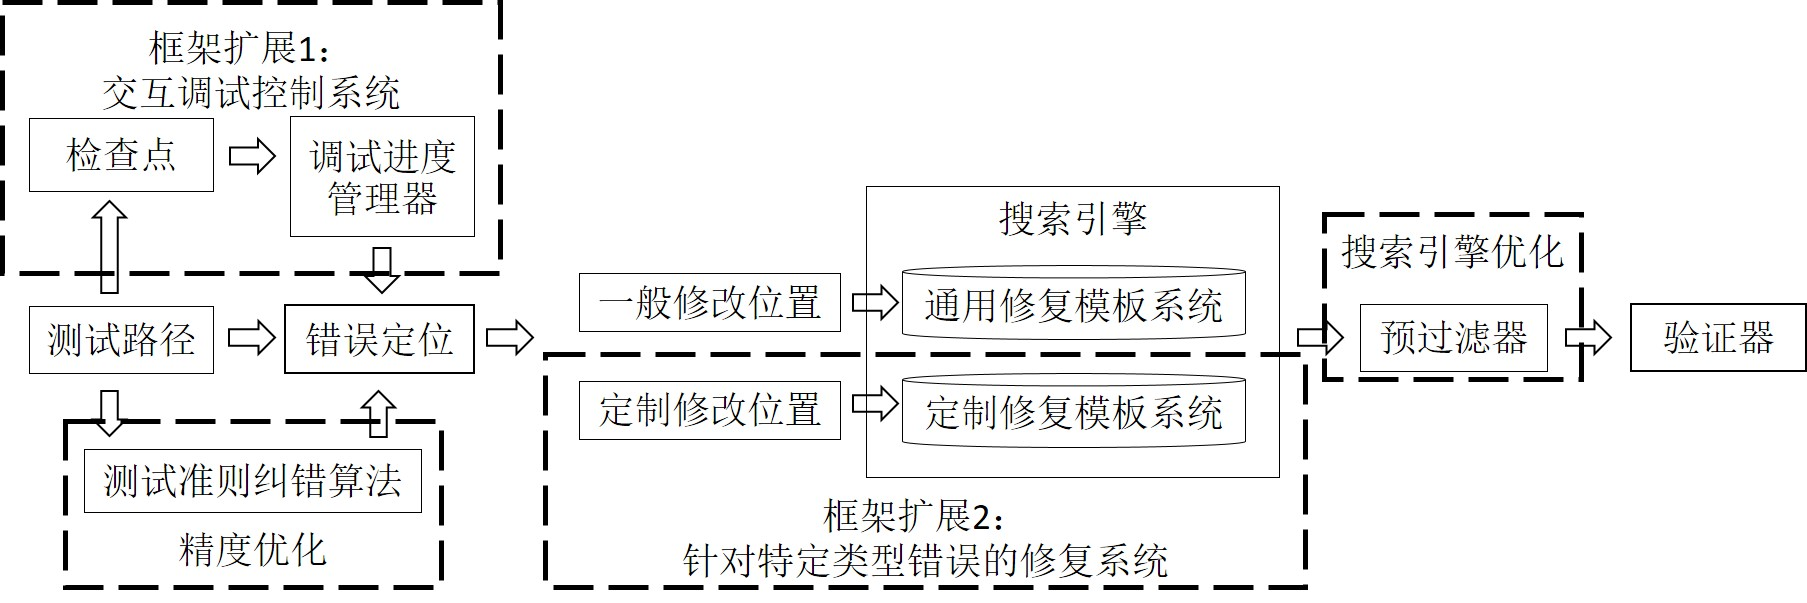
\includegraphics[width=1\linewidth]{chap01/roadmap}
	\caption{研究思路}
	\label{fig:roadmap}
\end{figure}

“生成-检验”系统研究的关键问题是如何提高系统的修复正确率与修复效率。图\ref{fig:roadmap}展示了本文的研究思路。本文首先着眼于系统框架内部,针对“生成-检验”系统工作流中的两个关键步骤进行性能优化。步骤一是“错误定位”。本文提出实际程序中测试准则可能并不完善,而这将使已有的错误定位算法精度降低。本文提出一种依据测试用例执行路径相似性判断及其测试结果识别测试准则错误的方法,使得在修正了被识别的测试准则后,已有错误定位算法精度恢复到原有水平,系统整体的修复效率不会受损。步骤二是“搜索修复方案”。本文提出当搜索引擎内部使用搜索模板系统定义搜索空间时,可以使用一种“预过滤”策略将搜索过程中生成的与表达式替换相关修复方案预先过滤、压缩,减少检验器最终需要验证的修复方案数目,提高系统整体效率。由于搜索速度提高,系统能够负担的搜索空间也相应扩大,系统的修复正确率也超过现有其他工作。

在上述工作基础上,本文提出在系统框架层面进一步扩充系统功能。本文提出了两种系统框架方案,第一种是引入开发人员与系统的交互,使得系统能够利用开发人员对程序运行状态的基本了解,更准确地定位错误,提高系统运行效率。第二种则是规范系统模块实现接口,使得开发者可以方便的在系统框架上进行二次开发,将针对特定类型的错误修复算法集成到系统中,与原系统形成优势互补。

总之,本文以提高系统的修复正确率和修复效率为目标,从模块层算法优化入手,以框架层改进方案为结束,对“生成-检验”框架进行了深入研究,具有系统性。

\section{论文贡献}

本文以基于“生成-检验”框架的程序错误自动修复算法为研究内容,从系统内部模块优化、系统框架扩展两个方面提出提高系统的修复正确率和效率的技术方案,最终形成原型工具SmartDebug。主要贡献如下:
\begin{enumerate}[1.]
	\item 提出不完全正确“测试准则”存在的普遍性,并以实验说明测试准则错误对“生成-检验”系统中常用的基于频谱的错误定位算法(SFL)错误定位精度的负面影响。针对这一问题,本文提出了一种基于测试用例执行路径相似性识别测试准则错误的算法。实验表明,算法能够识别出测试准则中的错误,并且SFL算法精度在修正后的测试准则下能够成功恢复。
	\item 针对搜索引擎中与表达式替换、修改相关的修复模板,提出“预过滤”策略,根据测试集中已通过和未通过的测试用例的运行时状态在备选修复方案进入到检验器前过滤掉其中不符合要求的修复方案,同时压缩搜索空间,减轻检验器的工作负担。实验表明,“预过滤”策略能够过滤掉搜索空间中约90\%的修复方案,使得系统效率大幅提升,系统整体修复正确率也超过现有的其他系统。
	\item 在系统框架层提出两种扩展方案。第一是提供使用者与系统交互的接口,使得系统能够利用使用者的经验减少无用搜索操作,提高系统效率。第二是提供二次开发接口,使得开发人员能够根据需求方便的引入针对特定类型错误的修复算法,使得系统本身的修复能力得到补充。
	\item 实现原型系统SmartDebug,系统中包含了本文提出的优化技术以及扩展框架,并集成在Eclipse平台中供开发者在日常开发过程中使用。
\end{enumerate}
%1)提高错误定位准确性的技术:Oracle debugging;

%2)本文提出“预过滤”技术优化搜索引擎,压缩搜索空间,提高搜索与验证效率,

%3)本文针对现有修复框架的缺陷提出两种扩展方式:a)“交互式调试”设计模式,即给用户提供方便的图形界面,使其能够依据自己的经验将调试任务分段处理。b)针对单类别错误的可扩展框架。本文整理了“生成-检验”框架,使其能够方便的融合针对单类别错误的修复算法,从而扩展修复工具的修复能力,使其能够利用已知类别错误的特异性提高修复准确率和效率。

%4)系统实现SmartDebug。SmartDebug以插件形式集成在Eclipse集成开发环境中,可供下载使用和二次开发。
\section{论文结构}%0.5

本文共分为6个章节,其中第二章介绍测试准则错误修正算法,第三章介绍“预过滤”算法,第四章介绍两种框架扩展方案,第五章介绍系统功能与使用案例,第六章总结本文工作并给出未来研究方向。
